\documentclass[11pt]{scrartcl}
\usepackage[utf8]{inputenc}

\usepackage{framed}
\usepackage{amsmath}
\usepackage{float}
\DeclareMathOperator\Arg{Arg}
\DeclareMathOperator{\arcsec}{arcsec}
\DeclareMathOperator{\arccot}{arccot}
\DeclareMathOperator{\arccsc}{arccsc}
\DeclareMathOperator{\trig}{trig}
\DeclareMathOperator{\arctrig}{arctrig}
\usepackage{graphicx}
\usepackage{array}

\title{Hackpack}
\author{Calcutta Kids}
\date{}



\usepackage{listings}
\usepackage{xcolor}

\definecolor{codegreen}{rgb}{0,0.6,0}
\definecolor{codegray}{rgb}{0.5,0.5,0.5}
\definecolor{codepurple}{rgb}{0.58,0,0.82}
\definecolor{backcolour}{rgb}{0.95,0.95,0.92}

\lstdefinestyle{mystyle}{
    backgroundcolor=\color{backcolour},   
    commentstyle=\color{codegreen},
    keywordstyle=\color{magenta},
    numberstyle=\tiny\color{codegray},
    stringstyle=\color{codepurple},
    basicstyle=\ttfamily\footnotesize,
    breakatwhitespace=false,         
    breaklines=true,                 
    captionpos=b,                    
    keepspaces=true,                 
    numbers=left,                    
    numbersep=5pt,                  
    showspaces=false,                
    showstringspaces=false,
    showtabs=false,                  
    tabsize=2
}

\lstset{style=mystyle}

\begin{document}




\maketitle

ASCII Table :pray:
\begin{figure}[H]
    \centering
    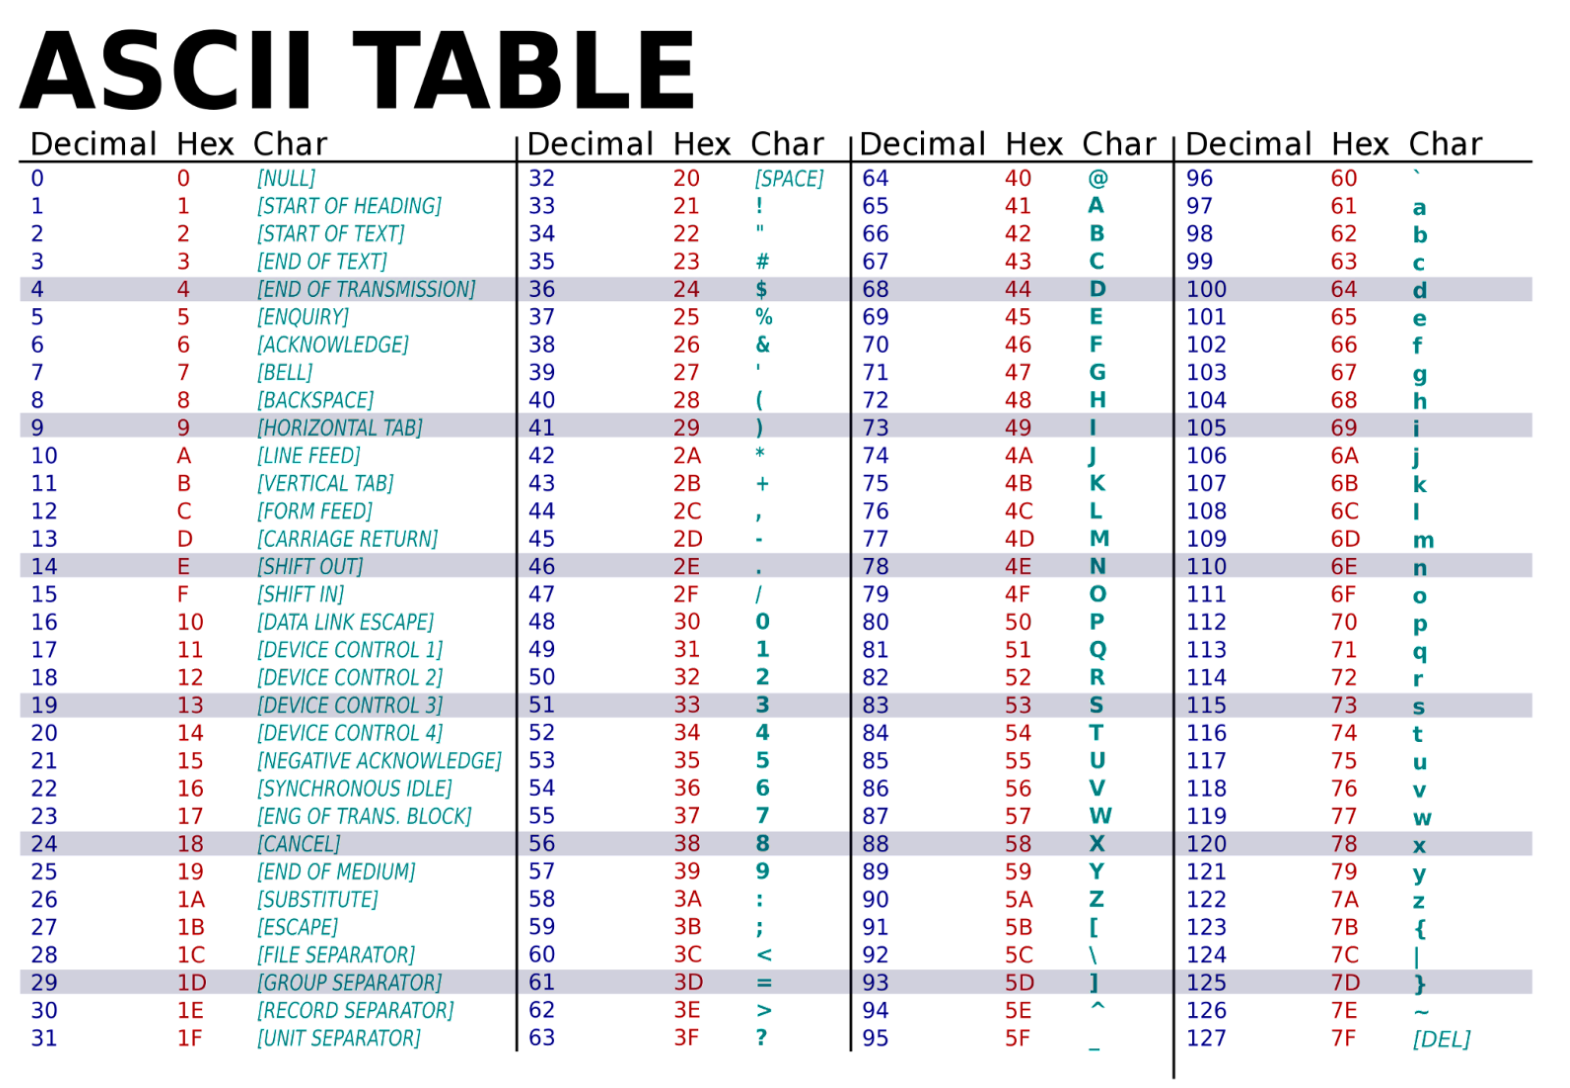
\includegraphics[width=12cm]{bob.png}
    \label{fig:my_label}
\end{figure}


\noindent UFDS
\begin{lstlisting}[language=Python]
function MakeSet(x) is
    if x is not already in the forest then
        x.parent := x
        x.size := 1     // if nodes store size
        x.rank := 0     // if nodes store rank
    end if
end function

function Find(x) is
    if x.parent ≠ x then
        x.parent := Find(x.parent)
        return x.parent
    else
        return x
    end if
end function

Or function Find(x) is
    root := x
    while root.parent ≠ root do
        root := root.parent
    end while

    while x.parent ≠ root do
        parent := x.parent
        x.parent := root
        x := parent
    end while

    return root
end function

Or function Find(x) is
    while x.parent ≠ x do
        (x, x.parent) := (x.parent, x.parent.parent)
    end while
    return x
end function

function Union(x, y) is
    // Replace nodes by roots
    x := Find(x)
    y := Find(y)

    if x = y then
        return  // x and y are already in the same set
    end if

    // If necessary, rename variables to ensure that
    // x has at least as many descendants as y
    if x.size < y.size then
        (x, y) := (y, x)
    end if

    // Make x the new root
    y.parent := x
    // Update the size of x
    x.size := x.size + y.size
end function

\end{lstlisting}
\vspace{5mm}
\noindent Kruskal's Minimum Spanning Tree - Java
\begin{lstlisting}[language=Java]
import java.util.*;
import java.lang.*;
import java.io.*;
 
class Graph {
    // A class to represent a graph edge
    class Edge implements Comparable<Edge>
    {
        int src, dest, weight;
 
        // Comparator function used for
        // sorting edges based on their weight
        public int compareTo(Edge compareEdge)
        {
            return this.weight - compareEdge.weight;
        }
    };
 
    // A class to represent a subset for
    // union-find
    class subset
    {
        int parent, rank;
    };
 
    int V, E; // V-> no. of vertices & E->no.of edges
    Edge edge[]; // collection of all edges
 
    // Creates a graph with V vertices and E edges
    Graph(int v, int e)
    {
        V = v;
        E = e;
        edge = new Edge[E];
        for (int i = 0; i < e; ++i)
            edge[i] = new Edge();
    }
 
    // A utility function to find set of an
    // element i (uses path compression technique)
    int find(subset subsets[], int i)
    {
        // find root and make root as parent of i
        // (path compression)
        if (subsets[i].parent != i)
            subsets[i].parent
                = find(subsets, subsets[i].parent);
 
        return subsets[i].parent;
    }
 
    // A function that does union of two sets
    // of x and y (uses union by rank)
    void Union(subset subsets[], int x, int y)
    {
        int xroot = find(subsets, x);
        int yroot = find(subsets, y);
 
        // Attach smaller rank tree under root
        // of high rank tree (Union by Rank)
        if (subsets[xroot].rank
            < subsets[yroot].rank)
            subsets[xroot].parent = yroot;
        else if (subsets[xroot].rank
                 > subsets[yroot].rank)
            subsets[yroot].parent = xroot;
 
        // If ranks are same, then make one as
        // root and increment its rank by one
        else {
            subsets[yroot].parent = xroot;
            subsets[xroot].rank++;
        }
    }
 
    // The main function to construct MST using Kruskal's
    // algorithm
    void KruskalMST()
    {
        // Tnis will store the resultant MST
        Edge result[] = new Edge[V];
       
        // An index variable, used for result[]
        int e = 0;
       
        // An index variable, used for sorted edges
        int i = 0;
        for (i = 0; i < V; ++i)
            result[i] = new Edge();
 
        // Step 1:  Sort all the edges in non-decreasing
        // order of their weight.  If we are not allowed to
        // change the given graph, we can create a copy of
        // array of edges
        Arrays.sort(edge);
 
        // Allocate memory for creating V subsets
        subset subsets[] = new subset[V];
        for (i = 0; i < V; ++i)
            subsets[i] = new subset();
 
        // Create V subsets with single elements
        for (int v = 0; v < V; ++v)
        {
            subsets[v].parent = v;
            subsets[v].rank = 0;
        }
 
        i = 0; // Index used to pick next edge
 
        // Number of edges to be taken is equal to V-1
        while (e < V - 1)
        {
            // Step 2: Pick the smallest edge. And increment
            // the index for next iteration
            Edge next_edge = edge[i++];
 
            int x = find(subsets, next_edge.src);
            int y = find(subsets, next_edge.dest);
 
            // If including this edge does't cause cycle,
            // include it in result and increment the index
            // of result for next edge
            if (x != y) {
                result[e++] = next_edge;
                Union(subsets, x, y);
            }
            // Else discard the next_edge
        }
 
        // print the contents of result[] to display
        // the built MST
        System.out.println("Following are the edges in "
                           + "the constructed MST");
        int minimumCost = 0;
        for (i = 0; i < e; ++i)
        {
            System.out.println(result[i].src + " -- "
                               + result[i].dest
                               + " == " + result[i].weight);
            minimumCost += result[i].weight;
        }
        System.out.println("Minimum Cost Spanning Tree "
                           + minimumCost);
    }
}

\end{lstlisting}

\vspace{5mm}
\noindent The weirdest BFS of all time
\begin{lstlisting}


   procedure BFS(G, root) is
       let Q be a queue
       label root as explored
       Q.enqueue(root)
       while Q is not empty do
           v := Q.dequeue()
           if v is the goal then
               return v
           for all edges from v to w in G.adjacentEdges(v) do
              if w is not labeled as explored then
                  label w as explored
                  Q.enqueue(w)

       //sky[][] is the map array we are searching on and visited[][] is the array of nodes already visited
       //”-” is the character we are searching for
   public static void find(int i, int j) {
 
      if(sky[i][j] == '-') visited[i][j]=true;
      if(sky[i+1][j] == '-' && !visited[i+1][j]) find(i+1, j);
      if(sky[i-1][j] == '-' && !visited[i-1][j]) find(i-1, j);
      if(sky[i][j+1] == '-' && !visited[i][j+1]) find(i, j+1);
      if(sky[i][j-1] == '-' && !visited[i][j-1]) find(i, j-1);
 
   }
 \end{lstlisting}
\vspace{5mm}
\noindent Dijkstarsd's(I think that's how you spell it) Shortest Path Theorem- C++
\begin{lstlisting}[language = c++]
#include <iostream>
using namespace std;
#include <limits.h>
 
// Number of vertices in the graph
#define V 9
 
// A utility function to find the vertex with minimum distance value, from
// the set of vertices not yet included in shortest path tree
int minDistance(int dist[], bool sptSet[])
{
   
    // Initialize min value
    int min = INT_MAX, min_index;
 
    for (int v = 0; v < V; v++)
        if (sptSet[v] == false && dist[v] <= min)
            min = dist[v], min_index = v;
 
    return min_index;
}
 
// A utility function to print the constructed distance array
void printSolution(int dist[])
{
    cout <<"Vertex \t Distance from Source" << endl;
    for (int i = 0; i < V; i++)
        cout  << i << " \t\t"<<dist[i]<< endl;
}
 
// Function that implements Dijkstra's single source shortest path algorithm
// for a graph represented using adjacency matrix representation
void dijkstra(int graph[V][V], int src)
{
    int dist[V]; // The output array.  dist[i] will hold the shortest
    // distance from src to i
 
    bool sptSet[V]; // sptSet[i] will be true if vertex i is included in shortest
    // path tree or shortest distance from src to i is finalized
 
    // Initialize all distances as INFINITE and stpSet[] as false
    for (int i = 0; i < V; i++)
        dist[i] = INT_MAX, sptSet[i] = false;
 
    // Distance of source vertex from itself is always 0
    dist[src] = 0;
 
    // Find shortest path for all vertices
    for (int count = 0; count < V - 1; count++) {
        // Pick the minimum distance vertex from the set of vertices not
        // yet processed. u is always equal to src in the first iteration.
        int u = minDistance(dist, sptSet);
 
        // Mark the picked vertex as processed
        sptSet[u] = true;
 
        // Update dist value of the adjacent vertices of the picked vertex.
        for (int v = 0; v < V; v++)
 
            // Update dist[v] only if is not in sptSet, there is an edge from
            // u to v, and total weight of path from src to  v through u is
            // smaller than current value of dist[v]
            if (!sptSet[v] && graph[u][v] && dist[u] != INT_MAX
                && dist[u] + graph[u][v] < dist[v])
                dist[v] = dist[u] + graph[u][v];
    }
 
    // print the constructed distance array
    printSolution(dist);
}
 
// driver program to test above function
int main()
{
   
    /* Let us create the example graph discussed above */
    int graph[V][V] = { { 0, 4, 0, 0, 0, 0, 0, 8, 0 },
                        { 4, 0, 8, 0, 0, 0, 0, 11, 0 },
                        { 0, 8, 0, 7, 0, 4, 0, 0, 2 },
                        { 0, 0, 7, 0, 9, 14, 0, 0, 0 },
                        { 0, 0, 0, 9, 0, 10, 0, 0, 0 },
                        { 0, 0, 4, 14, 10, 0, 2, 0, 0 },
                        { 0, 0, 0, 0, 0, 2, 0, 1, 6 },
                        { 8, 11, 0, 0, 0, 0, 1, 0, 7 },
                        { 0, 0, 2, 0, 0, 0, 6, 7, 0 } };
 
    dijkstra(graph, 0);
 
    return 0;
}

\end{lstlisting}

\vspace{5mm}
Dkjistrasds' shortest path theorem - Java
\begin{lstlisting}[language = java]
import java.util.*;
import java.lang.*;
import java.io.*;
 
class ShortestPath {
    // A utility function to find the vertex with minimum distance value,
    // from the set of vertices not yet included in shortest path tree
    static final int V = 9;
    int minDistance(int dist[], Boolean sptSet[])
    {
        // Initialize min value
        int min = Integer.MAX_VALUE, min_index = -1;
 
        for (int v = 0; v < V; v++)
            if (sptSet[v] == false && dist[v] <= min) {
                min = dist[v];
                min_index = v;
            }
 
        return min_index;
    }
 
    // A utility function to print the constructed distance array
    void printSolution(int dist[])
    {
        System.out.println("Vertex \t\t Distance from Source");
        for (int i = 0; i < V; i++)
            System.out.println(i + " \t\t " + dist[i]);
    }
 
    // Function that implements Dijkstra's single source shortest path
    // algorithm for a graph represented using adjacency matrix
    // representation
    void dijkstra(int graph[][], int src)
    {
        int dist[] = new int[V]; // The output array. dist[i] will hold
        // the shortest distance from src to i
 
        // sptSet[i] will true if vertex i is included in shortest
        // path tree or shortest distance from src to i is finalized
        Boolean sptSet[] = new Boolean[V];
 
        // Initialize all distances as INFINITE and stpSet[] as false
        for (int i = 0; i < V; i++) {
            dist[i] = Integer.MAX_VALUE;
            sptSet[i] = false;
        }
 
        // Distance of source vertex from itself is always 0
        dist[src] = 0;
 
        // Find shortest path for all vertices
        for (int count = 0; count < V - 1; count++) {
            // Pick the minimum distance vertex from the set of vertices
            // not yet processed. u is always equal to src in first
            // iteration.
            int u = minDistance(dist, sptSet);
 
            // Mark the picked vertex as processed
            sptSet[u] = true;
 
            // Update dist value of the adjacent vertices of the
            // picked vertex.
            for (int v = 0; v < V; v++)
 
                // Update dist[v] only if is not in sptSet, there is an
                // edge from u to v, and total weight of path from src to
                // v through u is smaller than current value of dist[v]
                if (!sptSet[v] && graph[u][v] != 0 && dist[u] != Integer.MAX_VALUE && dist[u] + graph[u][v] < dist[v])
                    dist[v] = dist[u] + graph[u][v];
        }
 
        // print the constructed distance array
        printSolution(dist);
    }
 
    // Driver method
    public static void main(String[] args)
    {
        /* Let us create the example graph discussed above */
        int graph[][] = new int[][] { { 0, 4, 0, 0, 0, 0, 0, 8, 0 },
                                      { 4, 0, 8, 0, 0, 0, 0, 11, 0 },
                                      { 0, 8, 0, 7, 0, 4, 0, 0, 2 },
                                      { 0, 0, 7, 0, 9, 14, 0, 0, 0 },
                                      { 0, 0, 0, 9, 0, 10, 0, 0, 0 },
                                      { 0, 0, 4, 14, 10, 0, 2, 0, 0 },
                                      { 0, 0, 0, 0, 0, 2, 0, 1, 6 },
                                      { 8, 11, 0, 0, 0, 0, 1, 0, 7 },
                                      { 0, 0, 2, 0, 0, 0, 6, 7, 0 } };
        ShortestPath t = new ShortestPath();
        t.dijkstra(graph, 0);
    }
}
\end{lstlisting}

\vspace{5mm}
LCS - CPP

\begin{lstlisting}[language = C++]
    /* Returns length of LCS for X[0..m-1], Y[0..n-1] */
int lcs(string &X, string &Y)
{
	int m = X.length(), n = Y.length();
	int L[m+1][n+1];

	/* Following steps build L[m+1][n+1] in bottom up
	fashion. Note that L[i][j] contains length of
	LCS of X[0..i-1] and Y[0..j-1] */
	for (int i=0; i<=m; i++)
	{
		for (int j=0; j<=n; j++)
		{
			if (i == 0 || j == 0)
				L[i][j] = 0;

			else if (X[i-1] == Y[j-1])
				L[i][j] = L[i-1][j-1] + 1;

			else
				L[i][j] = max(L[i-1][j], L[i][j-1]);
		}
	}

	/* L[m][n] contains length of LCS for X[0..n-1] and
	Y[0..m-1] */
	return L[m][n];
}

\end{lstlisting}


\begin{lstlisting}[language = C++]
    int bin(vector<int> arr,int a){
    int lo = 0;
    int hi = arr.size()-1;
    int prev = INT_MAX;
    int mid;
    if(arr.size()==1&&arr[0]>a) return 0;
    if(a<arr[0]) return 0;
    while(lo<=hi){
        if(lo+1==hi&&arr[lo]<a&&arr[hi]>a) return hi;
        mid = lo + (hi-lo)/2;
        if(arr[mid]==a) return -1;
        if(arr[mid]<a) lo = mid;
        else if(arr[mid]>a) hi = mid;
    }
    return -1;

}
int lengthOfLIS(vector<int>& arr){
    int prev = INT_MIN;
    vector<int> final;
    fr(i,arr.size()){
        if(arr[i]>prev){
            final.push_back(arr[i]);
            prev = arr[i];
        }
        else if(arr[i]<prev){
            int index = bin(final,arr[i]);
            if(index!=-1) final[index] = arr[i];
            if(index==final.size()-1) prev = arr[i];
        }
//        cout << "prev: "<< prev <<"\n";
    }
//    fr(i,final.size()) cout << final[i]<<" ";
//    cout << "\n";
    return final.size();

}
\end{lstlisting}



\end{document}
